\documentclass[aspectratio=169, 12pt]{beamer}

% --- 日语支持与字体设置 (推荐使用 LuaLaTeX 编译) ---
\usepackage{luatexja}
\usepackage{luatexja-fontspec}
% 设置主字体 (如果编译报错,可以尝试注释掉下面两行)
\setmainjfont{HaranoAjiMincho}
\setsansjfont{HaranoAjiGothic}

% --- 宏包 ---
\usepackage{amsmath}
\usepackage{amssymb}
\usepackage{amsthm}
\usepackage{mathrsfs}
\usepackage{graphicx} % 用于插入图片
\usepackage{tikz} % 添加这个宏包用于绘图
\usetikzlibrary{arrows.meta} % 为了更好看的箭头

% --- Beamer 主题设置 ---
\usetheme{Madrid}
\usecolortheme{beaver}
\usefonttheme{professionalfonts}

% --- 元数据 ---
\title[Steepest Descent]{Method of Steepest Descent \\ (最急降下法)}
\subtitle{Chapter 4.2.3 - 4.2.4}
\author{Andre YI}
\date{2025年11月26日}

% --- 自定义命令 ---
\newcommand{\norm}[1]{\left\lVert#1\right\rVert}
\newcommand{\inner}[2]{\langle #1, #2 \rangle}

\begin{document}

% --- 标题页 ---
\begin{frame}
    \titlepage
\end{frame}

% --- 目录 ---
\begin{frame}{目次}
    \tableofcontents
\end{frame}

% --- Section 1: 概念与推导 ---
\section{最急降下方向の導出}

\begin{frame}{目的と設定}
    関数 $f:\mathbb{R}^{n}\rightarrow\mathbb{R}$ を最小化する問題を考えます。
    
    小さなステップ幅 $\eta > 0$ が与えられたとき、関数値を最も減少させる\textbf{単位ベクトル} $\nu$ ($||\nu||=1$) を求めたいと思います。
    
    \vspace{0.3cm}
    \textbf{テイラー展開による1次近似}:
    \begin{equation}
        f(x^{0}+\eta\nu)-f(x^{0}) \approx \eta\langle\nabla f(x^{0}),\nu\rangle
    \end{equation}
    
    この右辺を最小化する $\nu$ を探します。
\end{frame}

\begin{frame}{最適な方向 $\nu^*$}
    Cauchy-Schwarz の不等式を用いると、最適な方向 $\nu^*$ は以下のように求まります。
    
    \begin{block}{最急降下方向 (Steepest Descent Direction)}
        \begin{equation}
            \nu^{*} = -\frac{\nabla f(x^{0})}{||\nabla f(x^{0})||}
        \end{equation}
    \end{block}

    \vspace{0.3cm}
    関数値の最大変化は近似的に:
    $$ f(x^{0}+\eta\nu^{*})-f(x^{0}) \approx -\eta ||\nabla f(x^{0})|| < 0 $$
\end{frame}

% --- Section 2: アルゴリズム ---
\section{アルゴリズムと収束性}

\begin{frame}{標準的な勾配降下法}
    ステップ幅を $\eta_{n}=\delta||\nabla f(x^{n})||$ ($\delta>0$) と仮定すると、以下の反復式が得られます。
    
    \begin{alertblock}{Prop 1.1: 標準的な勾配降下法}
        \begin{equation}
            x^{n+1} = x^{n} - \delta \nabla f(x^{n})
        \end{equation}
    \end{alertblock}

    \vspace{0.5cm}
    \textbf{収束性について}:
    $$ (x^{n})_{n} \text{ が収束} \iff \lim_{n\rightarrow\infty} \nabla f(x^{n}) = 0 $$
\end{frame}

\begin{frame}{パラメータ $\delta$ による挙動の違い:図示}
    $|1-\delta| < 1 \iff 0 < \delta < 2$ の範囲における $(x^n, y^n)$ の軌跡:

    \vspace{0.2cm}

    \begin{columns}[T] % T align aligns the top lines
        % --- 左侧:图 a (单调收敛) ---
        \begin{column}{0.48\textwidth}
            \centering
            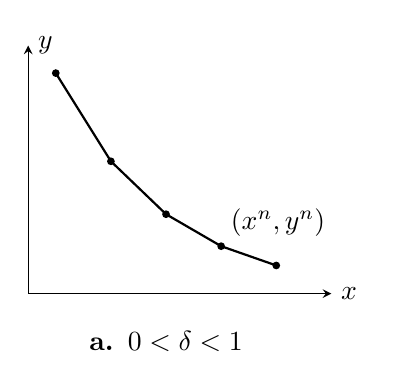
\begin{tikzpicture}[scale=0.7]
                % 坐标轴
                \draw[->, >=stealth] (0,0) -- (5.5,0) node[right] {$x$};
                \draw[->, >=stealth] (0,0) -- (0,4.5) node[right] {$y$};
                
                % 点列数据 (模拟 0 < delta < 1 的情况)
                \coordinate (A0) at (0.5, 4.0);
                \coordinate (A1) at (1.5, 2.4);
                \coordinate (A2) at (2.5, 1.44);
                \coordinate (A3) at (3.5, 0.86);
                \coordinate (A4) at (4.5, 0.51);

                % 连线与绘制点
                \draw[thick] (A0) -- (A1) -- (A2) -- (A3) -- (A4);
                \foreach \p in {A0,A1,A2,A3,A4} \fill (\p) circle (2pt);

                % 标签
                \node[above right] at (A3) {$(x^n, y^n)$};
                \node[below] at (2.5, -0.5) {\textbf{a. $0 < \delta < 1$}};
            \end{tikzpicture}
            
            \vspace{0.2cm}
            \footnotesize{単調に収束する (Monotonic)}
        \end{column}

        % --- 右侧:图 b (震荡收敛) ---
        \begin{column}{0.48\textwidth}
            \centering
            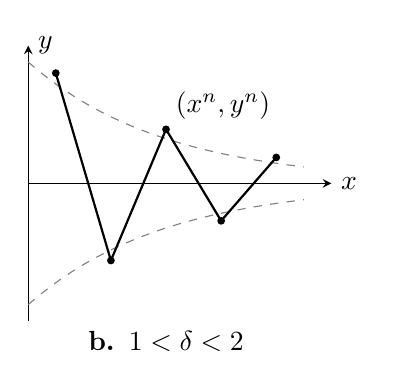
\begin{tikzpicture}[scale=0.7]
                % 坐标轴 (y轴居中)
                \draw[->, >=stealth] (0,0) -- (5.5,0) node[right] {$x$};
                \draw[->, >=stealth] (0,-2.5) -- (0,2.5) node[right] {$y$};

                % 包络线 (Envelope) - 虚线
                \draw[dashed, gray] plot[domain=0:5] (\x, {2.2*exp(-0.4*\x)});
                \draw[dashed, gray] plot[domain=0:5] (\x, {-2.2*exp(-0.4*\x)});

                % 点列数据 (模拟 1 < delta < 2 的情况,震荡)
                \coordinate (B0) at (0.5, 2.0);
                \coordinate (B1) at (1.5, -1.4);
                \coordinate (B2) at (2.5, 0.98);
                \coordinate (B3) at (3.5, -0.68);
                \coordinate (B4) at (4.5, 0.47);

                % 连线与绘制点
                \draw[thick] (B0) -- (B1) -- (B2) -- (B3) -- (B4);
                \foreach \p in {B0,B1,B2,B3,B4} \fill (\p) circle (2pt);

                % 标签
                \node[above right] at (B2) {$(x^n, y^n)$};
                \node[below] at (2.5, -2.5) {\textbf{b. $1 < \delta < 2$}};
            \end{tikzpicture}
            
            \vspace{0.2cm}
            \footnotesize{振動しながら収束する (Oscillating)}
        \end{column}
    \end{columns}
\end{frame}

% --- Appendix / 結び ---
\section{まとめ}

\begin{frame}{まとめ}
    \begin{itemize}
        \item \textbf{最急降下法}: $-\nabla f$ 方向へ進む。
        \item \textbf{勾配降下法}: $x^{n+1} = x^{n} - \delta \nabla f(x^{n})$。
        \item \textbf{ステップ幅 $\delta$ の重要性}:
            \begin{itemize}
                \item 適切ならスムーズに収束 (図 a)。
                \item 大きすぎると振動が発生 (図 b)。
            \end{itemize}
    \end{itemize}
    
    \vspace{1cm}
    \centering
    \large{ご清聴ありがとうございました。}
\end{frame}

\end{document}